\documentclass{beamer}

% Some common packages
\usepackage{graphicx, color}
\usepackage{alltt}
\usepackage{booktabs, calc, rotating}
\usepackage[round]{natbib}
\usepackage{multicol}
\usepackage{amsmath, amsbsy, amssymb, amsthm, graphicx}
\usepackage[english]{babel}
\usepackage{xkeyval} 
\usepackage{xfrac}
\usepackage[normalem]{ulem}
\usepackage{fancyvrb} 
\usepackage{tikz, geometry, tkz-graph, xcolor}
\usepackage[latin1]{inputenc}
\usepackage{times}
\usepackage[T1]{fontenc}

% Shortcuts
\newcommand{\empr}[1]{{\emph{\color{red}#1}}}
\newcommand{\cov}{\mathrm{cov}}
\newcommand{\pkg}[1]{{\textbf{\texttt{#1}}}}
\newcommand{\dif}{\mathrm{d}}
\newcommand{\bigbrk}{\vspace*{2in}}
\newcommand{\smallbrk}{\vspace*{.1in}}
\newcommand{\midbrk}{\vspace*{1in}}
\newcommand{\red}[1]{{\color{red}#1}}
\newcommand{\blue}[1]{{\color{blue}#1}}
\newcommand{\green}[1]{{\color{green}#1}}
\newcommand{\calc}[1]{{\fbox{\mbox{#1}}}}
\newcommand{\Var}{\mathrm{Var}}%
\newcommand{\Cov}{\mathrm{Cov}}%

\mode<presentation>
{
	\usetheme{UTD}
	\usecolortheme[RGB={200,0,0}]{structure}
	\setbeamercovered{transparent}
}

% fancy for Verbatim?
\fvset{frame=single,framesep=1mm,fontfamily=courier,fontsize=\scriptsize,numbers=left,framerule=.3mm,numbersep=1mm,commandchars=\\\{\}}


\title[Survival Analysis]{Applied Survival Analysis Using R\\ Chapter 3: Nonparametric Survival Curve Estimation}
\author[Qi Guo]{Qi Guo}
\institute[UTD]{Department of Mathematical Sciences \\ 
	The University of Texas at Dallas}
\date{April, 10 2019}
	
\begin{document}

\begin{frame}
  \titlepage
\end{frame}

% Set up UTD backgroud
\setbeamercolor*{item}{fg=red}
\bgroup
\usebackgroundtemplate{
\tikz[overlay,remember picture] \node[opacity=0.05, at=(current page.center)] {
   
\includegraphics[height=\paperheight,width=\paperwidth]{UTDbg}};}


\section[Outline]{}
\begin{frame}
  \tableofcontents
\end{frame}

\section{Kaplan-Meier estimator}
\begin{frame}
\frametitle{Kaplan-Meier estimator}
\begin{itemize}
\item  In this chapter we will discuss non-parametric estimators of the survival function
\end{itemize}

\begin{defblock}{Kaplan-Meier estimator}
\empr{KM estimator} is the product over the failure times of the conditional probabilities of surviving to the next failure time.
\end{defblock}

\begin{itemize}
\item Formally, it given by:
\end{itemize}

\begin{equation}
\hat{S}(t)=\prod\limits_{t_i\le t}^{}(1-\hat{q_i})=\prod\limits_{t_i\le t}^{}(1 - \frac{d_i}{n_i})
\end{equation}

\begin{itemize}
	\item where $n_i$ is the number of subjects {\color{red} at risk} at time $t_i$, and $d_i$ is the number of {\color{red} individuals who fail} at that time, so $q_i = \frac{d_i}{n_i}$ is {\color{red}failure probability}
\end{itemize}	
\end{frame}

\pagebreak
\begin{frame}
\frametitle{Example}
\begin{itemize}
\item The example data in \texttt{Table 1.1} may be used to illustrate the construction of the \empr{KM estimate}, as shown in \texttt{Table 3.1} .	
\end{itemize}
\begin{figure}[t]
	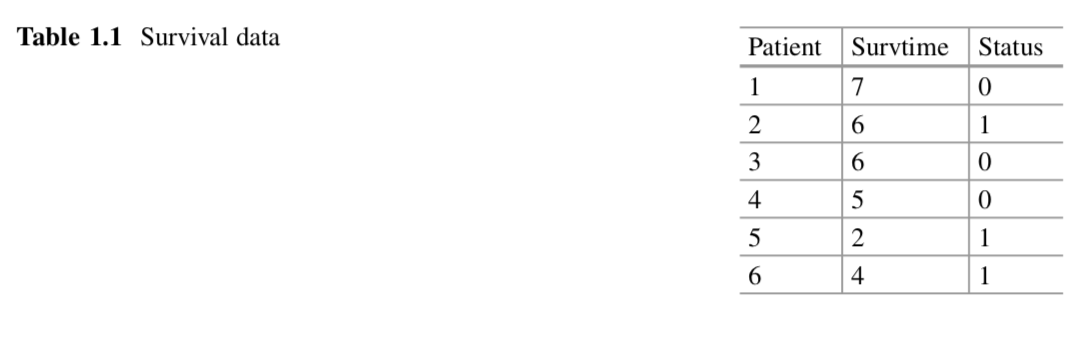
\includegraphics[scale = .3]{001.png}
	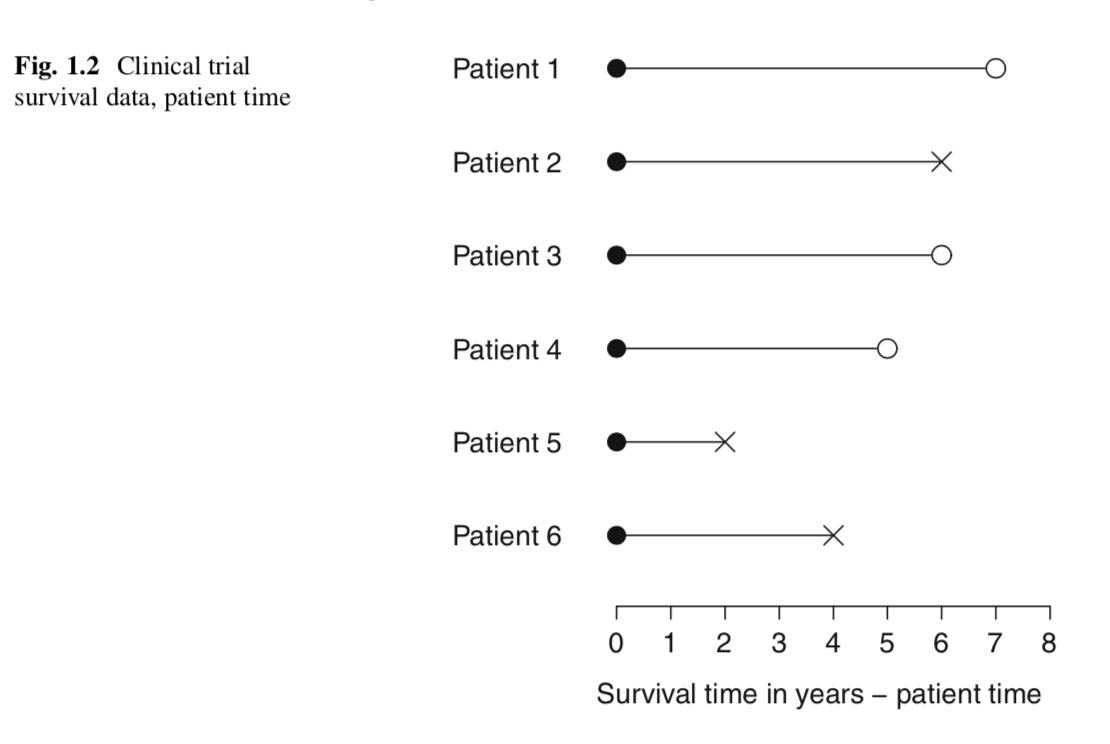
\includegraphics[scale = .3]{002.png}
\end{figure}
\end{frame}

\pagebreak
\begin{frame}
\frametitle{Get Variance By Delta Method}
\begin{itemize}
\item To obtain confidence limits for the product-limit estimator, we first use what is known as the ``\pkg{delta method}''  to obtain the variance of $log(\hat{S}(t))$
\end{itemize}
\begin{equation}
var(\log(\hat{S}(t_k))) = \sum\limits_{t_i\le t}^{}var(\log(1-\hat{q_i}))\approx \sum\limits_{t_i\le t}^{} \frac{d_i}{n_i(n_i -d_i)}
\end{equation}

\begin{itemize}
\item To get the variance of $\hat{S}(t)$ itself, we use the delta method again to obtain:
\end{itemize}
\begin{equation}
var(\hat{S}(t_k))\approx [\hat{S}(t)]^{2} \sum\limits_{t_i\le t}^{} \frac{d_i}{n_i(n_i -d_i)}
\end{equation}
\end{frame}

\pagebreak
\begin{frame}
\frametitle{log-log transformation}
\begin{itemize}
\item A more satisfying approach is to find confidence intervals for the complementary \empr{log-log transformation} of $\hat{S}(t)$  as follows:
\end{itemize}
\begin{equation}
var(\log([-\log\hat{S}(t_k)])\approx \frac{1}{[\log\hat{S}(t)]^{2}}\sum\limits_{t_i\le t}^{} \frac{d_i}{n_i(n_i -d_i)}
\end{equation}
\end{frame}

\pagebreak
\begin{frame}[fragile]
\frametitle{R}
\begin{itemize}
\item To obtain estimates of the \empr{Kaplan-Meier estimator} in \texttt{R} for the data in \texttt{Table 1.1}, we first load the  ``\pkg{survival}'' library, and then enter the data
\end{itemize}

\begin{Verbatim}
> library(survival)
> tt <- c(7,6,6,5,2,4)
> cens <- c(0,1,0,0,1,1)
> Surv(tt, cens)
[1] 7+  6   6+  5+  2  4
\end{Verbatim}

\begin{itemize}
\item For the estimation itself we use the ``\pkg{survfit}'' function
\end{itemize}

\begin{Verbatim}
> result.km <- survfit(Surv(tt, cens) ~ 1, conf.type="log-log")
> result.km
[1] records   n.max   n.start   events   median   0.95LCL  0.95UCL 
       6        6        6        3         6        2        NA
\end{Verbatim}
\end{frame}

\pagebreak
\begin{frame}[fragile]
\frametitle{R}
\begin{itemize}
\item To see the full \empr{Kaplan-Meier estimate}, and plot it, we use the  ``\pkg{summary}'' and ``\pkg{plot}'' functions:
\end{itemize}

\begin{Verbatim}
> summary(result.km)
[1]
time   n.risk   n.event  survival   std.err   lower95%CI   upper95%CI
2        6       1      0.833       0.152       0.2731       0.975
4        5       1      0.667       0.192       0.1946       0.904
6        3       1      0.444       0.222       0.0662       0.785

> plot(result.km)
\end{Verbatim}
\begin{figure}[h!]
	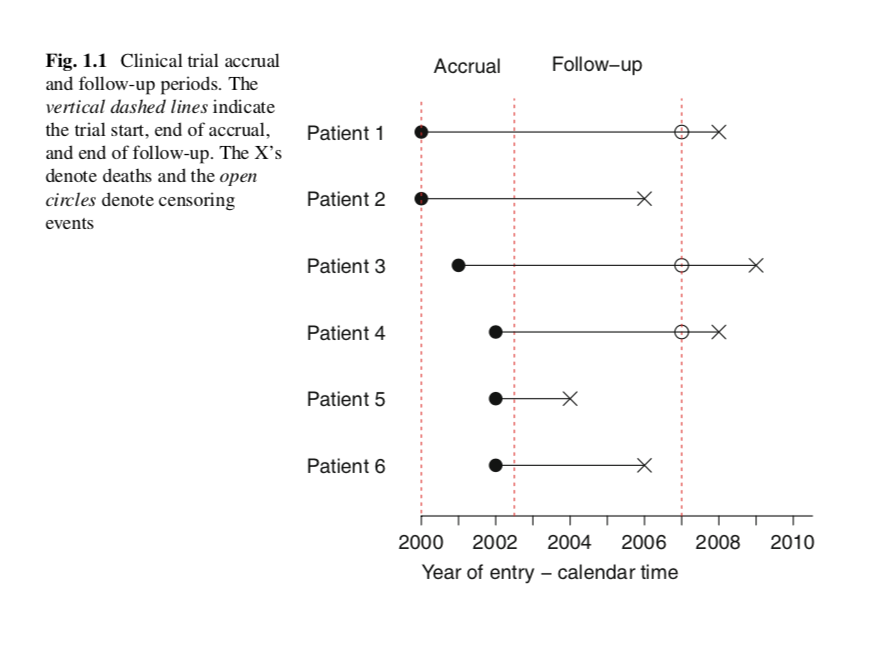
\includegraphics[scale = .25]{003.png}
\end{figure}
\end{frame}

\section{Nelson-Aalen Estimator}
\begin{frame}
\frametitle{Nelson-Aalen Estimator}
\begin{itemize}
\item Based on the {\color{red}relationship} of {\color{red}$S(t)$} and {\color{red}$h(t)$}. 
\item An estimate of the cumulative hazard function is the {\color{red}sum} of the estimated {\color{red}hazards up to a time $t_i$}: 
\end{itemize}
\begin{equation}
H(t) =  \sum\limits_{t_i\le t}^{}\frac{d_i}{n_i}
\end{equation}
\begin{itemize}
\item and the \empr{survival function} estimate is simply
\end{itemize}
\begin{equation}
S(t) =  e^{-H(t)}
\end{equation}
\end{frame}	

\pagebreak
\begin{frame}[fragile]
\frametitle{R}
\begin{itemize}
\item \empr{The Nelson-Aalen estimate} may be obtained using the ``\pkg{survfit}'' function with the option \texttt{type = ``fh''}
\end{itemize}
\begin{Verbatim}
> result.fh <- survfit(Surv(tt, cens) ~ 1, conf.type="log-log",
 type="fh")
> summary(result.fh)
[1]
time   n.risk   n.event  survival   std.err   lower95%CI   upper95%CI
  2       6       1      0.846       0.155       0.2401       0.981
  4       5       1      0.693       0.200       0.1799       0.925
  6       3       1      0.497       0.248       0.0585       0.841
\end{Verbatim}
\end{frame}

\section{The Median Survival and a Confidence Interval for the Median}
\begin{frame}
\frametitle{Median and CI for Median}
\begin{itemize}
\item Formally, the median survival time may be defined as:
 ${\hat{t}}_{med} = \inf \lbrace t : \hat{S}(t)\le 0.5\rbrace $
\end{itemize}
\begin{itemize}
\item To find a $1-\alpha$ confidence interval for the median:
\end{itemize}
\begin{equation}
-z_{\alpha/2} \le \frac{g\lbrace\hat{S}(t)\rbrace-g(0.5)}{\sqrt{var[g\lbrace\hat{S}(t)\rbrace]}}\le z_{\alpha/2}
\end{equation}

\begin{itemize}
\item where $g(\mu)=\log[-\log(\mu)]$ and $var[g\lbrace\hat{S}(t)\rbrace]$ is given by equation (4)
\end{itemize}
\end{frame}

\section{Left Truncation}
\begin{frame}
\frametitle{Left Truncation}

\begin{defblock}{Left Truncation}
Instead of examining the time from {\color{red}entry} into the clinical trial until {\color{red}censoring or death}, let us use as the time origin the time of {\color{red}diagnosis}.
\end{defblock}

\begin{figure}[h!]
	\includegraphics[scale = .35]{004.png}
\end{figure}
\end{frame}


\pagebreak
\begin{frame}
\frametitle{Figure}
\begin{figure}[h!]
\includegraphics[scale = .3]{005.png}
\includegraphics[scale = .3]{006.png}
\end{figure}
\begin{itemize}
	\item We have used the terms ``\pkg{tm.enter}'' and ``\pkg{tm.exit}'' for the \empr{left truncation} and \empr{survival times}, respectively.
\end{itemize}
\end{frame}

\pagebreak
\begin{frame}[fragile]
\frametitle{R}
\begin{Verbatim}
> tt <- c(7, 6, 6, 5, 2, 4)
> status <- c(0, 1, 0, 0, 1, 1)
> backTime <- c(-2, -5, -3, -3, -2, -5)
> tm.enter <- -backTime
> tm.exit <- tt - backTime
> result.left.trunc.km <- survfit(Surv(tm.enter, tm.exit, status, 
type="counting") ~ 1,  conf.type = "none")
> summary(result.left.trunc.km) 
[1]
time   n.risk   n.event  entered   censored   survival   std.err
 4        4        1        0         0        0.750       0.217
 9        4        1        0         2        0.562       0.230
11        1        1        0         0        0.000        NAN
> result.left.trunc.naa <- survfit(Surv(tm.enter, tm.exit, status, 
type="counting") ~ 1, type="fleming-harrington", conf.
type="none")
> summary(result.left.trunc.naa)
[1]
time   n.risk   n.event  entered   censored   survival   std.err
4        4        1        0         0        0.779       0.225
9        4        1        0         2        0.607       0.248
11       1        1        0         0        0.223        Inf
\end{Verbatim}
\end{frame}


\section{Example}
\begin{frame}[fragile]
\frametitle{Data}
\begin{itemize}
\item A serious problem arises with \empr{left-truncated data} if the risk set becomes \empr{empty at an early survival time}.
\item Consider for example the \empr{Channing House data}, ``\texttt{ChanningHouse}''. 
\item This data is subject to \empr{left truncation} because subjects who die at {\color{red}older ages} are {\color{red}more likely} to have enrolled in the center than patients who died at {\color{red}younger ages}.
\end{itemize}

\begin{Verbatim}
> head(ChanningHouse)
[1] sex     entry    exit     time    cens
1 Male       782      909      127      1
2 Male      1020     1128      108      1
3 Male       856      969      113      1
4 Male       915      957       42      1
5 Male       863      983      120      1
6 Male       906     1012      106      1
\end{Verbatim}
\end{frame}

\pagebreak
\begin{frame}[fragile]
\frametitle{Transform data and using KM and NAA estimator}
\begin{itemize}
\item Transform the data 
\end{itemize}
\begin{Verbatim}
>ChanningHouse <- within(ChanningHouse, 
{entryYears <- entry/12 
exitYears <- exit/12})
>ChanningMales <- ChanningHouse[ChanningHouse$sex == "Male",]
\end{Verbatim}
\begin{itemize}
\item {\color{red}KM estimator}
\end{itemize}
\begin{Verbatim}
>result.km <- survfit(Surv(entryYears, exitYears, cens, 
type="counting") ~ 1, data=ChanningMales)
>plot(result.km, xlim=c(64, 101), xlab="Age",
ylab="Survival probability", conf.int=F)
\end{Verbatim}
\begin{itemize}
\item {\color{red}NAA estimator}
\end{itemize}
\begin{Verbatim}
>result.naa <- survfit(Surv(entryYears, exitYears, cens,
type="counting") ~ 1, type="fleming-harrington",
data=ChanningMales)
>lines(result.naa, col="blue", conf.int=F)
\end{Verbatim}
\end{frame}

\pagebreak
\begin{frame}[fragile]
\frametitle{KM.68 and Plot}
\begin{itemize}
\item Men reach the age of 68, using the ``\texttt{start.time}'' option: 
\end{itemize}
\begin{Verbatim}
>result.km.68 <- survfit(Surv(entryYears, exitYears, cens,
type="counting") ~ 1, start.time=68, data=ChanningMales)
\end{Verbatim}
\begin{itemize}
\item Plot
\end{itemize}
\begin{Verbatim}
> lines(result.km.68, col="green", conf.int=F)
> legend("topright", legend=c("KM", "NAA", "KM 68 and older"),
lty=1, col=c("black", "blue", "green"))
\end{Verbatim}
\end{frame}


\pagebreak
\begin{frame}
\frametitle{Plot}
\begin{figure}[h!]
	\includegraphics[scale = .4]{007.png}
\end{figure}
\begin{itemize}
\item Apparently, \empr{the KM 68 and older} is much {\color{red}better behaved}.
\end{itemize}
\end{frame}
\end{document}